\documentclass[12pt, letterpaper]{article}
\usepackage[utf8]{inputenc}
\usepackage[letterpaper, margin=1.5in]{geometry}
\usepackage{siunitx}
\usepackage{amsmath}
\usepackage{amssymb}
\usepackage{graphicx}

\title{Fully Convolutional Segmentation of Lung Nodules in CT/PET Scans}
\author{Jonathan Lee, Gerald Wu}
\date{\today}

\begin{document}
	\maketitle
	\section{Introduction}
	Lung cancer represents a major health problem. Lung cancer is the formation of a malignant tumor in the lungs, caused by uncontrolled growth of cells in the tissue. According to the Center for Disease Control (CDC), lung cancer is the third most common cancer, and results in the highest number of deaths -- 1.3 million deaths annually according to the World Health Organization (WHO).\par
	Early detection of tumors in the lung could potentially help a significant number of people. Currently, CT and PET scans are used frequently to detect and diagnose lung cancer. As the resolution of these scans increase, physicians can view high-resolution volumetric scans, which describe lung anatomy and pathology. However, the increased resolution may also increase the difficulty of segmenting the tumors. We aim to automate this process by using deep learning to segment out portions PET and CT scans that look like tumors.
	\section{Methodology}
	\subsection{Preprocessing}
	\begin{figure}[h]
		\centering
		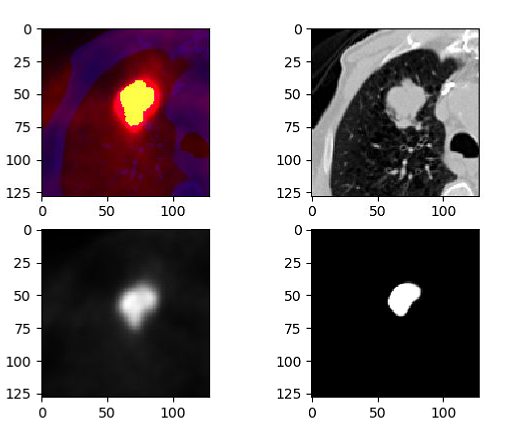
\includegraphics[width=0.65\textwidth]{img/segment.png}
		\caption[caption]{\\\hspace{\textwidth}\textbf{Top left}: CT, PET, ground truth label combined data\\\hspace{\textwidth}\textbf{Top right}: CT scan\\\hspace{\textwidth}\textbf{Bottom left}: PET scan\\\hspace{\textwidth}\textbf{Bottom right}: Our model's segmentation data}
		\label{fig:segment}
	\end{figure}
To process the images, we first imported the DICOM scans to Python using PyDICOM. Then, we rescaled the voxels using the rescale slope and rescale intercept. We then converted the voxel scale to $1\times1\times1\si{\milli\meter\cubed}$ using trilinear interpolation in the SciPy library. We did this for every patient, which included a PET scan, CT scan, and tumor ground truth mask. As seen in Figure~\ref{fig:segment}, the PET, CT, and mask all line up in 3D space. For the CT scan, we normalized the value between 0 and 1 by linearly taking values between [-1000, 400]. Anything below was set to 0, and anything above was set to 1. This is justified, because anything below 1000 represents air, and anything above 400 represents bone. For the PET scans, we normalized by dividing each value by the maximum voxel intensity. However, some were negative due to integer overflow, so we set all the negatives to 1. Because our network couldn’t train on the whole scan due to memory constraints, we cut up the scans into $128\times128\times128\si{\milli\meter\cubed}$ cubes. To do this, we found the maximum and minimum (x,y,z) coordinates and randomly cut out a cube around them with a padding of 12 voxels -- unless the tumor was too large, in which case we simply let the tumor extend out of the cube. We let the network train on these cubes.
	\subsection{Network Architecture}
	The network was based on U-net, an encoder-decoder convolutional neural network, with residual and skip connections to classify the data. The encoder network is used to shrink the image in order to aggregate semantic information. In particular, our encoder network uses pre-activation residual blocks. These non-linear residuals are element-wise added to the input, which allows the network to utilize deeper architectures and improves the gradient flow. The residual blocks are 3x3x3 convolutional layers, preceded by instance normalization and Leaky ReLU. The residual blocks are only used in the encoder.\par
	The decoder network afterwards reconstructs the image, while using the aggregated semantic information extracted by the encoder network. In contrast to the encoder, the decoder network does not use any residual connections. Instead, we simply increase the resolution by using a trilinear upsampling at each layer. Then, we perform a 3x3x3 convolution after the upsampling that halves the number of feature maps.\par
	The skip connection transfers feature maps from encoder layers to their respective decoder layers in order to further enhance precise segmentation and semantic information. After each encoder output is concatenated to its respective decoder input, the network performs a 3x3x3 convolution to recombine the semantic with the localization information. Then, a 1x1x1 convolution halves the feature maps. This is repeated 5 times to bring our final layer down to an 8x8x8 image from the original 128x128x128 image.\par
	Due to all these layers and large 3D convolutions, GPU memory was a contentious resource. As a result, batch sizes were kept very small to prevent memory overflow -- normally a size of 2. Therefore, we used instance normalization, as it is more effective than batch normalization for such small batch sizes.\par
	\subsection{Loss}
	The network architecture lends itself to possible short-circuits, one of which is learning the identity function through the first layer’s encoder-decoder skip connection. To mitigate this, we implemented two additional loss layers, which are trained on the down-sampled ground-truth masks from lower layers. All these loss layers were weighted-summed together to compute the total loss $(\text{total loss} = \text{first layer loss} + 0.5 \cdot \text{second layer loss} + 0.25 \cdot \text{third layer loss})$. As a result, the network is forced to learn not only from its top layer, but also from lower layers. Each loss layer uses a soft dice loss, as this loss accurately determines the quality of a segmentation at each layer.\par
	\section{Challenges}
	Preprocessing was very challenging. We had two datasets -- in one dataset, the PET scans had no information on spacing between scans, therefore we couldn’t resample it and the dataset was unusable. We wanted to segment the lungs to help the network learn by removing the extraneous information in the tissue outside the lungs. We tried to do this with topological closing, but there were many times in which the air in the lungs was connected to the air outside due to artifacts in the scan. Therefore, this method was inconsistent at best, and we had to give up on segmenting the lung before segmenting the tumor.\par
	In addition, there is no soft dice loss in keras, so we had to create our own soft dice loss function. While it wasn’t too difficult to implement, the loss function determines the efficacy of the network. Along a similar thread, we tried using binary crossentropy loss. However, the class imbalance between tumor and non-tumor biased the crossentropy loss to make the network output all non-tumor. We tried to implement weighted binary crossentropy, but had difficulties and ultimately ended up using soft dice loss as our final loss function.\par
Soft dice loss doesn’t have the best gradient flow, so training doesn’t go very smoothly. With a learning rate of 0.0001, we only saw a decrease in loss after around 100 epochs. However, our training set was small, so we probably slightly overfit on our data set. Additionally, in segmentation, there is no one good metric of how good the segmentation is. Usually in these types of projects, a radiologist manually compares the results to what they believe is a good segmentation. However, neither of us are radiologists.\par
	In our case, cross validation is difficult because we don’t have much memory to run on the test set. Therefore, to run the test set, we would have to do batch sizes of 2, which would take a significant amount of time. Additionally, as mentioned previously, there is no one good metric we could use to cross validate the model. We did not have enough time to come up with a good solution to this problem, as most time was spent on preprocessing and training the model.
	\section{Results}
Refer to Figure~\ref{fig:segment}. This is an example of a segmentation generated by our model. As you can see, the generated segmentation matches quite well with the given ground truth label.\par
Refer to Figure~\ref{fig:loss}. This is a graph of our loss over 100 epochs. As mentioned before, the soft dice loss is unstable, so it frequently jumps all over the place. However, you can see an overall decreasing trend in the graph.
	\begin{figure}[h]
		\centering
		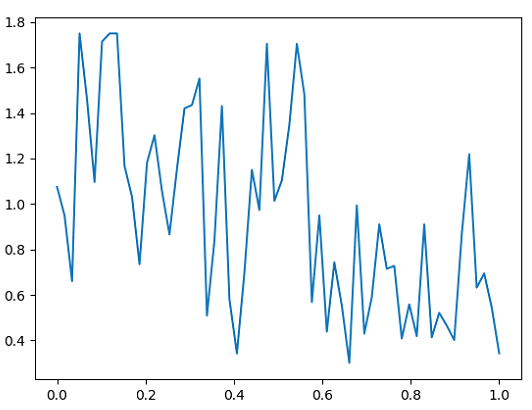
\includegraphics[width=0.5\textwidth]{img/loss.png}
		\caption{A graph of the loss over 100 epochs of training}
		\label{fig:loss}
	\end{figure}
	\section{Reflection}
In the future, we need to devise some way to cross-validate it, since our training set is so small. In addition, we can use data augmentation to increase the size of the data set. Additionally, we can filter the data for quality assurance, as some of the masks were incorrect, and some of the scans looked significantly different when compared to others. Along the same vein, we can sort the tumors into different sizes, so we can train the network on a more standard size tumor, which would allow much more fruitful training when compared to randomly sized tumors. Our dataset was primarily circular tumors, which means that the few tumors that were not circular did not have as high quality of a mask when put through the network. Additionally, we could try the weighted binary crossentropy, as the gradient flow is nicer than that of the soft dice loss. We had a lot of fun learning and writing this project. Thanks for a great semester!



\end{document}
